Researchers, service providers and security analysts have long been interested
in network and user behavioral patterns of the traffic crossing the internet
backbone. They want to use this information for the purpose of billing and
mediation, bandwidth provisioning, detecting malicious attacks, network
performance evaluation and overall improvement. Traffic measurement techniques
that have been rapidly evolving in the last decade, have matured enough today
to provide such an insight.

Flow capture today, has emerged out to be one of the favored network
measurement techniques. This has largely been due to the reduction in the
monitoring traffic at the flow-level and the fine-grained control which was
not previously possible using SNMP interface-level queries. As a result,
each networking vendor has tried to come up with a standard protocol that
defines the semantics of this flow export. In this pursuit, Cisco eventually
managed to make their proprietary protocol so ubiquitously available, that the
next-generation universal standard is based on it.

\todo{...}

\begin{figure*}[!t]
\centering
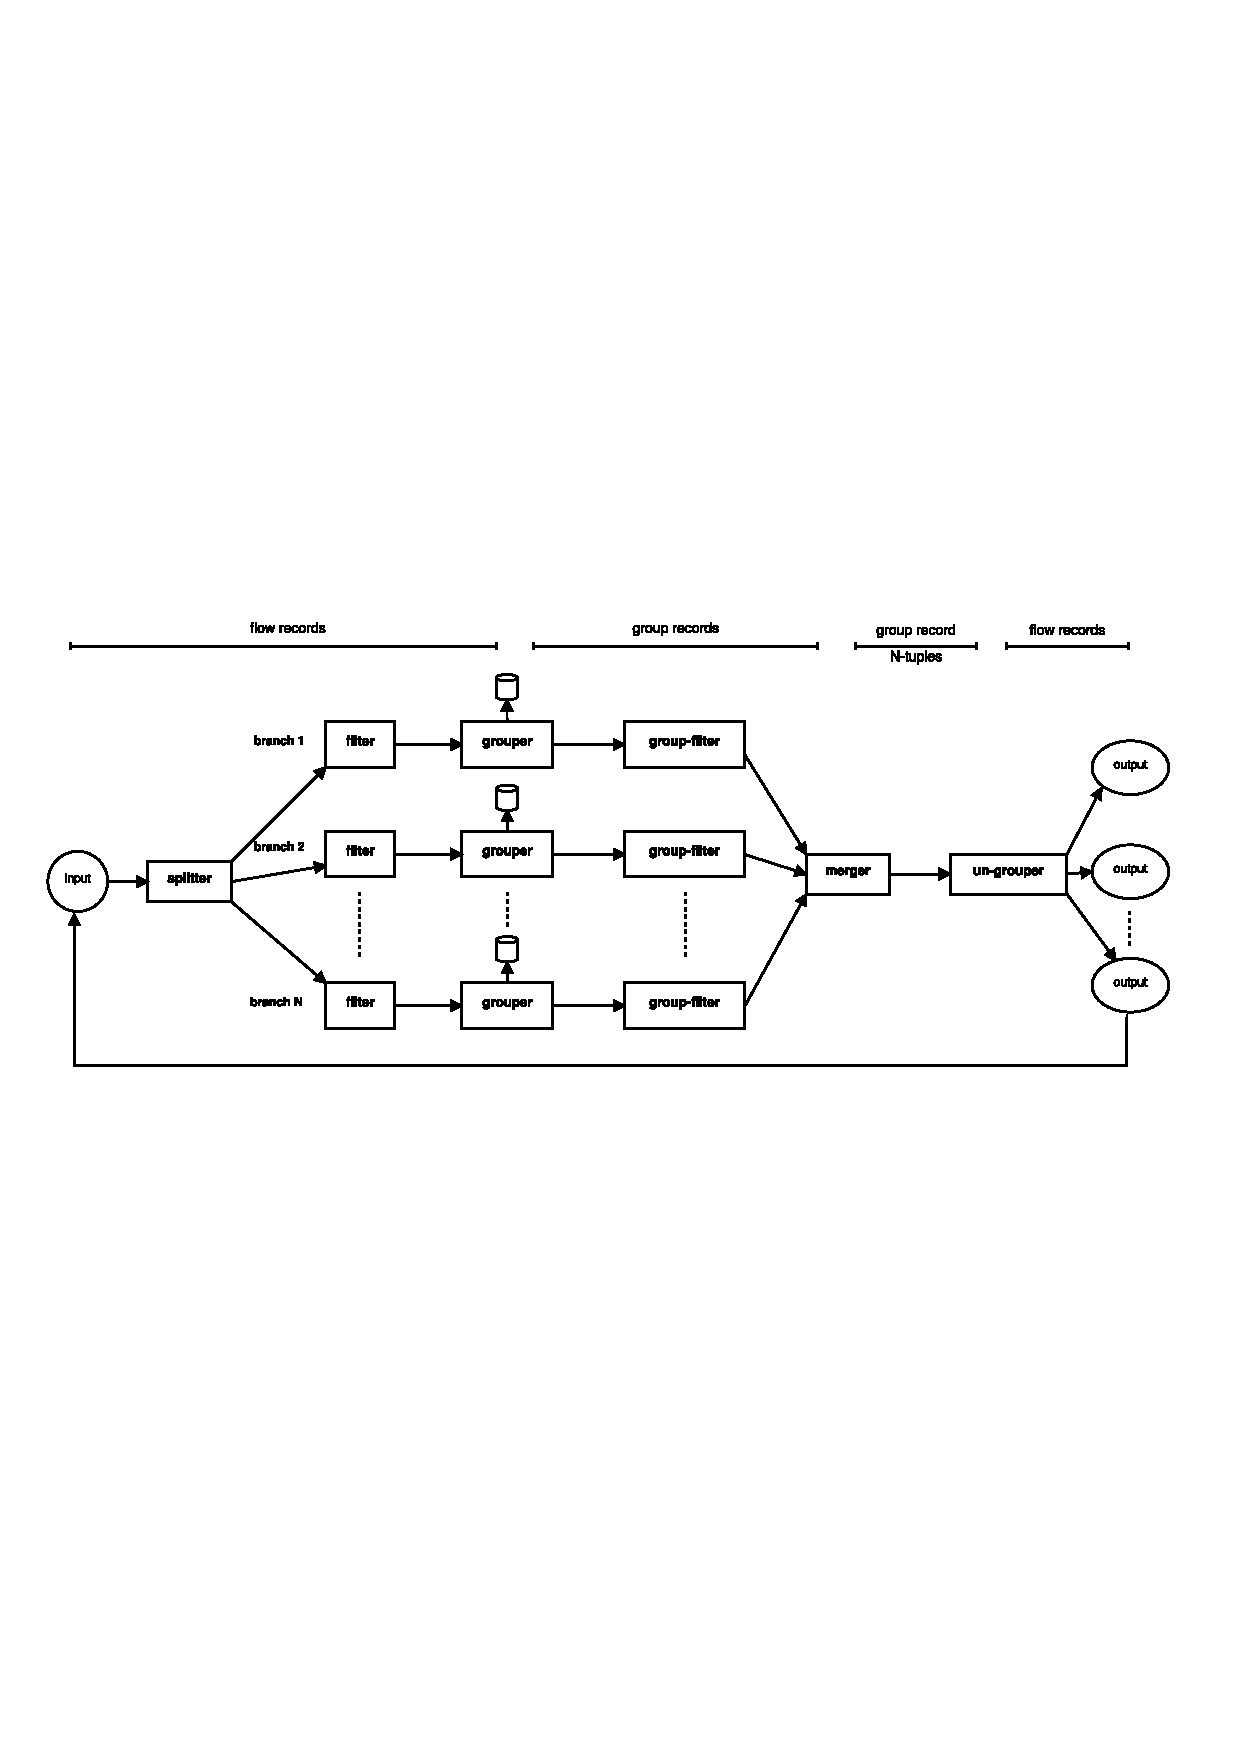
\includegraphics[width=1.0\linewidth]{nfql-pipeline}
\caption{NFQL Pipeline \cite{vmarinov:2009}}
\label{fig:nfql-pipeline}
\end{figure*}
